\chapter{Terms of Reference}

\section*{Description}

\begin{figure}[H]
\centering
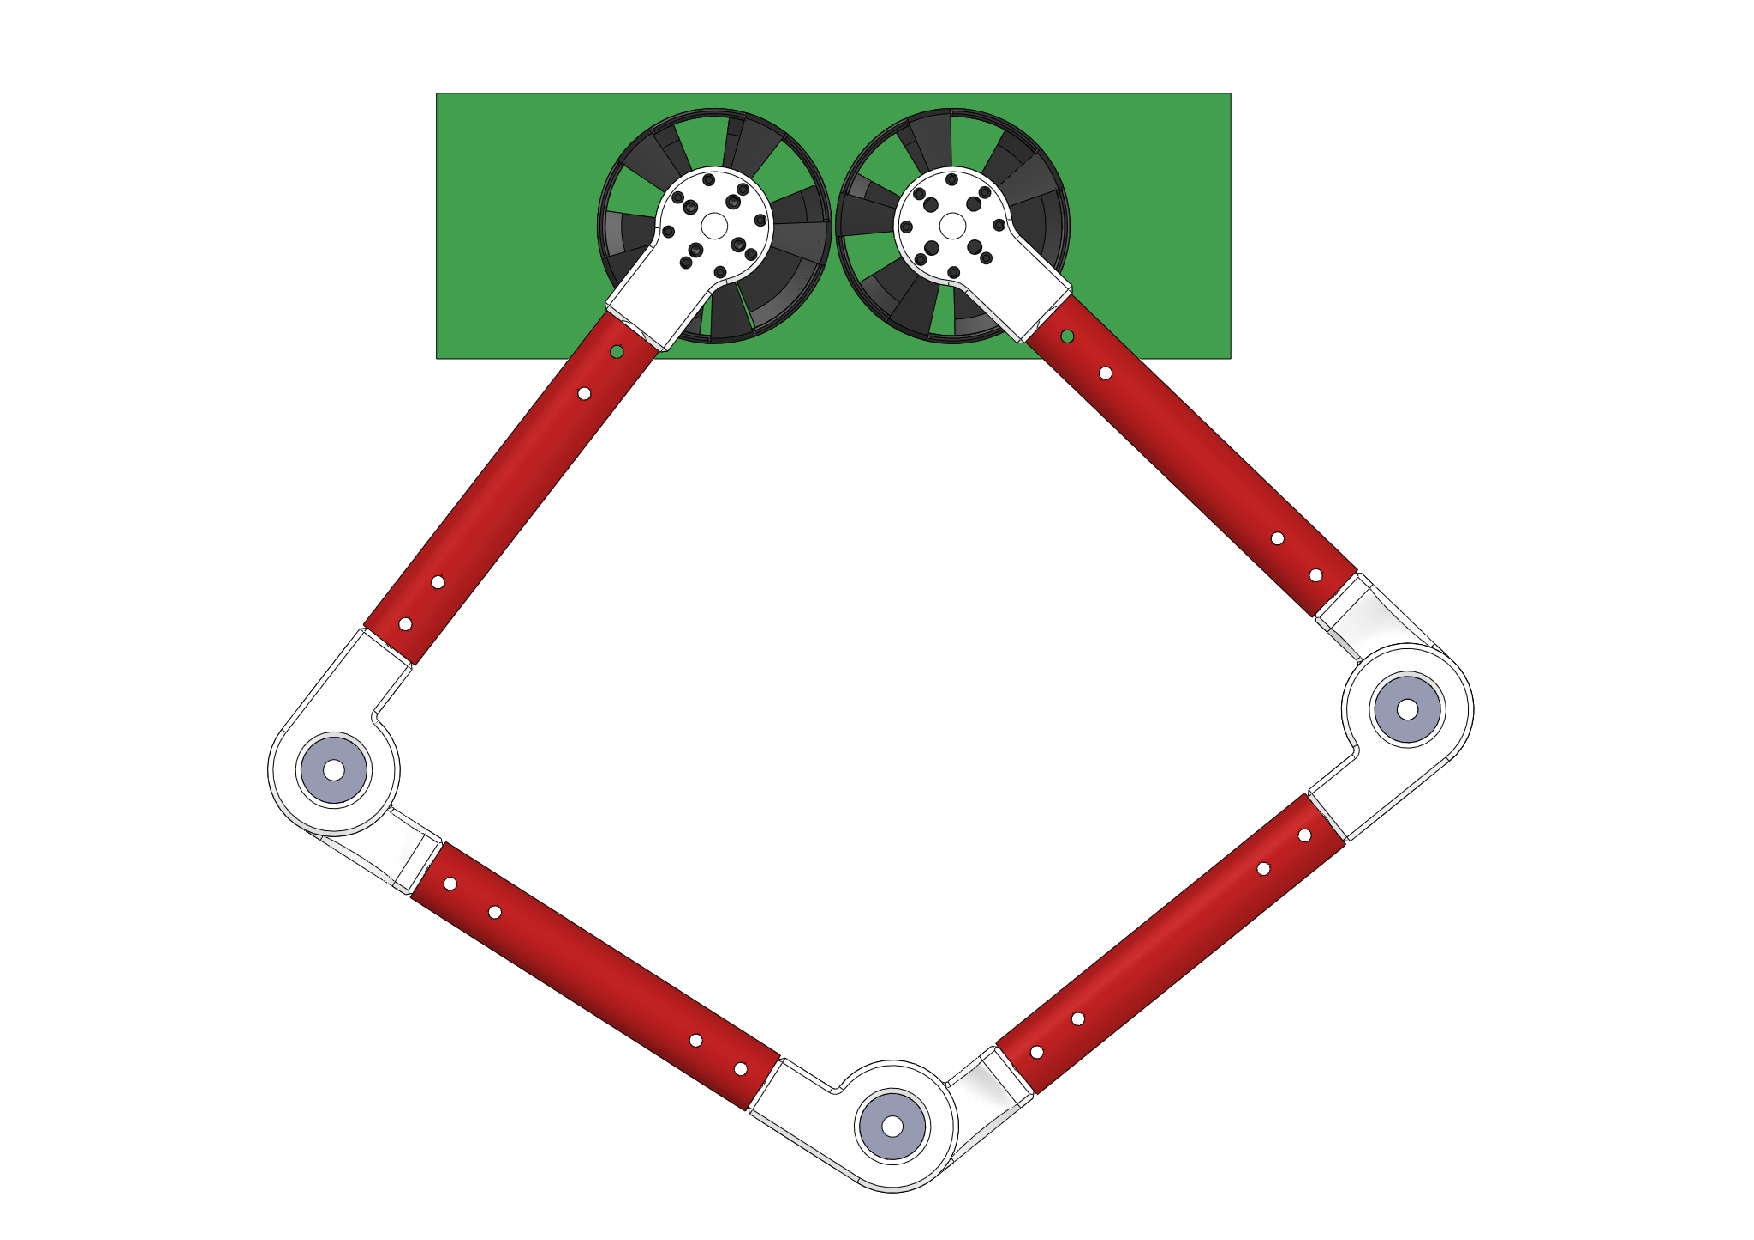
\includegraphics[width=0.7\textwidth,trim={0cm 0cm 0cm 0cm},clip]{images/mechanical/legsV1.pdf}
\caption{Version 1 of Baleka leg platform (Ben Bingham, 2016).}
\label{fig:legV1}
\end{figure}

The Mechatronics Lab has recently developed a single leg, direct drive robot,
Baleka, to investigate modelling and control of rapid accelerations.
This project will involve the design of a control system to perform stable
hopping with the robot. Various controller algorithms will be investigated and
compared (eg. PID, MPC, etc.). The project will also involve developing a test
rig for the robot.

\section*{Deliverables}

\begin{itemize}
\item Mathematical model of the hopping robot must be developed in
Simulink/Matlab
\item Hopping controller design
\item Mechanical design of the test rig
\item Experimental testing of the robot
\end{itemize}

\section*{Skills/Requirements}

\begin{itemize}
\item Mathematical Modelling 
\item Mechatronics Design
\item Control Systems
\item Embedded Systems
\item Strong Practical and Mathematical skills required
\end{itemize}

\section*{ELO3: Engineering Design}

\textit{Perform creative, procedural and non-procedural design and synthesis of components, systems, engineering works, products or processes.}

The student is expected to design:

\begin{itemize}
\item Robot feedback control system
\item Rig for testing of hopping motion
\end{itemize}

\section*{Area of Research}

\begin{itemize}
\item Bio-inspired robotics
\item Control systems
\end{itemize}

\section*{Extra Information}

\url{http://ieeexplore.ieee.org/xpls/abs_all.jsp?arnumber=5648972}

\url{http://kodlab.seas.upenn.edu/uploads/Avik/compositionTR_sc.pdf}
